\mysection{Résultats}
\mysubsection{Scripts}
Ci-dessous les résultats issus des scripts crées dans la troisième partie du projet suivis d'une bref discussion. 

\begin{itemize}
\item $\mathbf{gain\_calc-generator2bus}$\\
\begin{itemize}
	
\item $\mathbf{gain\_calc-generator2bus-test\_1-7am}$
\begin{table}[H]
	\captionsetup{justification=centering,margin=2cm}
	\caption{Matrice des Gain entre Puissance Réactive des générateurs et la tension des Bus ( Valeurs numériques )}
	\centering
	\begin{tabular}{ccc}
		1.7e-4&1.7e-4&1.7e-4\\
		1.7e-4&2.5e-4&2.7e-4\\
		1.7e-4&3.1e-4&2.4e-4\\
	\end{tabular}
\end{table}

\item $\mathbf{gain\_calc-generator2bus-test\_1-1pm}$
\begin{table}[H]
	\captionsetup{justification=centering,margin=2cm}
	\caption{Matrice des Gain entre Puissance Réactive des générateurs et la tension des Bus ( Valeurs numériques )}
	\centering
	\begin{tabular}{ccc}
		1.7e-4&1.7e-4&1.6e-4\\
		1.7e-4&2.4e-4&2.7e-4\\
		1.7e-4&3.0e-4&2.4e-4\\
	\end{tabular}
	
\end{table}
\newpage\vspace{2em}
\item $\mathbf{gain\_calc-generator2bus-test\_2}$
\begin{table}[H]
	\captionsetup{justification=centering,margin=2cm}
	\caption{Matrice des Gain entre Puissance Réactive des générateurs et la tension des Bus ( Valeurs numériques )}
	\centering
	\begin{tabular}{ccc}
		
		1.8e-4&1.8e-4&1.7e-4\\
		
		1.8e-4&2.5e-4&2.8e-4\\
		
		1.8e-4&3.1e-4&2.5e-4\\
	\end{tabular}
\end{table}\vspace{2em}
\item $\mathbf{gain\_calc-load2bus}$\\
\\A cause de sa taille, le tableau des résultats \ref{tab:matrice_gain_load2bus} sont dans une autre page.
\\
\end{itemize}\vspace{2em}
\item $\mathbf{teste\_simul}$\\
\\ Testé sans régulateur on peut voir le gain négative du système dans les figures  \ref{fig:Puissance_Active_et_Reactive_de_la_Charge_C2_29_MT} et \ref{fig:Tension_des_Bus_N21_N23_et_N29}.\\
\begin{minipage}{.475\textwidth}
\begin{figure}[H]
	\begin{center}
		\captionsetup{justification=centering,margin=.5cm}	
		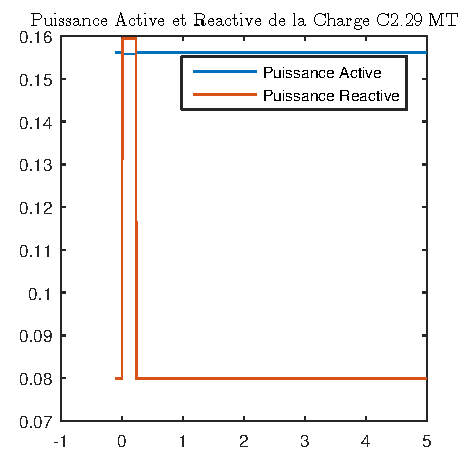
\includegraphics[width=\textwidth]{Resultats/Puissance_Active_et_Reactive_de_la_Charge_C2_29_MT.pdf}
		\caption{Puissance Active et Réactive \\de la Charge C2 29 MT}
		\label{fig:Puissance_Active_et_Reactive_de_la_Charge_C2_29_MT}
	\end{center}
\end{figure}
\end{minipage}
\begin{minipage}{.475\textwidth}
\begin{figure}[H]
	\begin{center}
		\captionsetup{justification=centering,margin=.5cm}	
		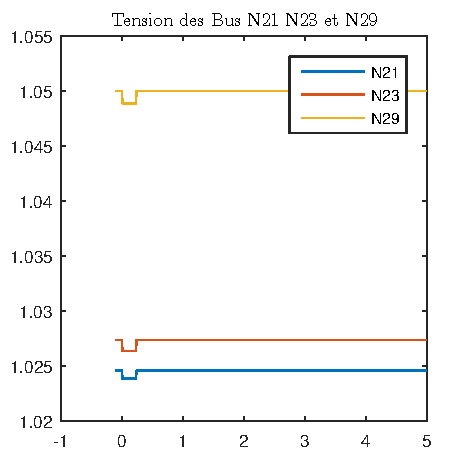
\includegraphics[width=\textwidth]{Resultats/Tension_des_Bus_N21_N23_et_N29.pdf}
		\caption{Tension des Bus N21 N23 et N29 en p.u.}
		\label{fig:Tension_des_Bus_N21_N23_et_N29}
	\end{center}
\end{figure}
\end{minipage}
\end{itemize}

\begin{sidewaysfigure}
	\begin{table}[H]\tiny
		\captionsetup{justification=centering,margin=2cm}
		\caption{Matrice des Gain entre Puissance Réactive des charges et la tension des Bus}
		\label{tab:matrice_gain_load2bus}
		\centering
		\resizebox{\textwidth}{!}{\begin{tabular}{ccccccccccccccccc}
				%	1&2&3&4&5&6&7&8&9&10&11&12&13&14&15&16\\
				0e+0& -9.0e-5& -1.1e-4& -1.1e-4& -1.1e-4& -1.1e-4& -1.1e-4& -1.1e-4& -1.1e-4& -1.1e-4& -1.1e-4& -1.1e-4& -1.1e-4& -1.1e-4& -1.1e-4& -1.1e-4\\
				0e+0& -8.9e-5& -1.1e-4& -1.3e-4& -1.3e-4& -1.3e-4& -1.3e-4& -1.3e-4& -1.3e-4& -1.3e-4& -1.3e-4& -1.3e-4& -1.3e-4& -1.3e-4& -1.3e-4& -1.3e-4\\
				0e+0& -9.1e-5& -1.1e-4& -1.3e-4& -1.8e-4& -1.8e-4& -1.8e-4& -1.8e-4& -1.8e-4& -1.8e-4& -1.8e-4& -1.8e-4& -1.8e-4& -1.8e-4& -1.8e-4& -1.8e-4\\
				0e+0& -1.2e-4& -1.5e-4& -1.8e-4& -2.5e-4& -3.5e-4& -4.2e-4& -4.2e-4& -4.2e-4& -4.2e-4& -4.2e-4& -3.4e-4& -3.4e-4& -3.4e-4& -3.4e-4& -3.4e-4\\
				0e+0& -9.4e-5& -1.2e-4& -1.4e-4& -1.9e-4& -2.7e-4& -3.3e-4& -3.9e-4& -3.9e-4& -3.9e-4& -3.9e-4& -2.6e-4& -2.6e-4& -2.6e-4& -2.6e-4& -2.6e-4\\
				0e+0& -9.5e-5& -1.2e-4& -1.4e-4& -1.9e-4& -2.7e-4& -3.3e-4& -4.0e-4& -4.3e-4& -4.3e-4& -4.3e-4& -2.7e-4& -2.6e-4& -2.6e-4& -2.7e-4& -2.7e-4\\
				0e+0& -9.3e-5& -1.2e-4& -1.4e-4& -1.9e-4& -2.6e-4& -3.2e-4& -3.8e-4& -4.2e-4& -4.5e-4& -4.5e-4& -2.6e-4& -2.6e-4& -2.6e-4& -2.6e-4& -2.6e-4\\
				0e+0& 0e+0& 0e+0& 0e+0& 0e+0& 0e+0& 0e+0& 0e+0& 0e+0& 0e+0& 0e+0& 0e+0& 0e+0& 0e+0& 0e+0& 0e+0\\
				0e+0& 0e+0& 0e+0& 0e+0& 0e+0& 0e+0& 0e+0& 0e+0& 0e+0& 0e+0& 0e+0& 0e+0& 0e+0& 0e+0& 0e+0& 0e+0\\
				0e+0& -9.7e-5& -1.2e-4& -1.4e-4& -2.0e-4& -2.7e-4& -3.4e-4& -4.0e-4& -4.4e-4& -4.8e-4& -5.2e-4& -2.7e-4& -2.7e-4& -2.7e-4& -2.7e-4& -2.7e-4\\
				0e+0& -9.5e-5& -1.2e-4& -1.4e-4& -1.9e-4& -2.7e-4& -2.7e-4& -2.7e-4& -2.7e-4& -2.7e-4& -2.7e-4& -2.8e-4& -2.8e-4& -2.8e-4& -2.8e-4& -2.8e-4\\
				0e+0& -9.1e-5& -1.1e-4& -1.3e-4& -1.9e-4& -2.6e-4& -2.6e-4& -2.6e-4& -2.6e-4& -2.6e-4& -2.6e-4& -2.7e-4& -2.8e-4& -2.8e-4& -2.9e-4& -2.9e-4\\
				0e+0& -9.5e-5& -1.2e-4& -1.4e-4& -1.9e-4& -2.7e-4& -2.7e-4& -2.7e-4& -2.7e-4& -2.7e-4& -2.7e-4& -2.8e-4& -3.0e-4& -3.1e-4& -3.1e-4& -3.1e-4\\
				0e+0& -9.3e-5& -1.2e-4& -1.4e-4& -1.9e-4& -2.6e-4& -2.6e-4& -2.7e-4& -2.7e-4& -2.7e-4& -2.7e-4& -2.8e-4& -2.9e-4& -3.1e-4& -3.2e-4& -3.2e-4\\
				0e+0& 0e+0& 0e+0& 0e+0& 0e+0& 0e+0& 0e+0& 0e+0& 0e+0& 0e+0& 0e+0& 0e+0& 0e+0& 0e+0& 0e+0& 0e+0\\
				0e+0& -9.2e-5& -1.2e-4& -1.4e-4& -1.9e-4& -2.6e-4& -2.6e-4& -2.6e-4& -2.6e-4& -2.6e-4& -2.6e-4& -2.8e-4& -2.9e-4& -3.0e-4& -3.2e-4& -3.4e-4
				\\
		\end{tabular}}
	\end{table} 
	
\end{sidewaysfigure}
\vspace{2em}
On peut voir a partir de ces données que le réseau est caractérisée pour les équations démontrés en \cite{cosson:tel-01374469}, la tension du bus a un gain positif par rapport à puissance réactive du générateur,  dû à l'injection de puissance et un gain négatif par rapport a puissance réactive des charges, dû à la consommation de puissance réactive. La variation de signal indique la production/consommation de puissance réactive.
\newpage
\mysubsection{Simulations avec le régulateur}
Comme les réponses étaient les mêmes entre les modèles Powerfactory,\\ Powerfactory$ \leftrightarrows $MATLAB et Powerfactory$ \leftrightarrows $MATLAB$ \leftrightarrows $Simulink, on a choisi d'afficher les résultats du modèle Powerfactory$ \leftrightarrows $MATLAB, afin d'avoir encore la communication entre les deux logiciels.

 Ici se présentent les réponses des simulations et après une bref discussion sur les résultats.
 
 Les premiers tests étaient pendant un intervalle de $ 50s $ et sans perturbations juste pour voir se le système reste avec sa tension dans la zone permise, ça veut dire entre $ \pm 5\% $ du valeur de tension nominal, $ 20kV $, donc l'intervalle est entre $ 19kV $ et $ 21kV $. Et on varie le paramètre $ a $ du filtre a fin de voir la différence induite sur le système.
 
 \vspace{2em}
 \begin{minipage}{.475\textwidth}
 \begin{figure}[H]
 	\begin{center}
 		\captionsetup{justification=centering,margin=.5cm}	
 		\includegraphics[width=\textwidth]{"Resultats/discrete_control/sans_perturbation/Tension_de_GD4_GD5_et_GD6_a0_4"}
 		\caption{Tension de GD4 sans perturbation $ a =0.4$.}
 		\label{fig:Tension_de_GD4_GD5_et_GD6_a0_4}
 	\end{center}
 \end{figure}
\end{minipage}
 \begin{minipage}{.475\textwidth}
 \begin{figure}[H]
 	\begin{center}
 		\captionsetup{justification=centering,margin=.5cm}	
 		\includegraphics[width=\textwidth]{"Resultats/discrete_control/sans_perturbation/Tension_de_GD4_GD5_et_GD6_a0_5"}
 		\caption{Tension de GD4 sans perturbation $ a =0.5$.}
 		\label{fig:Tension_de_GD4_GD5_et_GD6_a0_5}
 	\end{center}
 \end{figure}
 \end{minipage}

 \begin{figure}[H]
 	\begin{center}	
 		\includegraphics[width=.475\textwidth]{"Resultats/discrete_control/sans_perturbation/Tension_de_GD4_GD5_et_GD6_a0_6"}
 		\caption{Tension de GD4 sans perturbation $ a =0.6$.}
 		\label{fig:Tension_de_GD4_GD5_et_GD6_a0_6}
 	\end{center}
 \end{figure}
\newpage
On peut voir que le régulateur fonctionne, parce que les valeurs de tension restent dans l'intervalle proposé, et on peut percevoir que quand le paramètre $ a $ est plus proche de $ 0 $ le comportement du système commence a être oscillatoire.

Après ces tests, deux autres tests ont été faits, les deux avec perturbations a une charge (C2-29), le premier avec un échelon de puissance réactive et le seconde avec un échelon de puissance active. Les deux augmentent en $ 50\% $. Comme les réponses des trois générateurs sont semblables, juste les réponses d'un générateur sont montrées dans les figures suivantes afin de faciliter la visualisation.

%\begin{minipage}{.475\textwidth}
%	\begin{figure}[H]
%		\begin{center}	
%			\includegraphics[width=\textwidth]{"Resultats/discrete_control/avec_perturbation/puissance_charge/Tension_et_Puissance_Reactive_de_GD4_P50_a0_4"}
%			\caption{\todo{escrevaaquiseucaption}}
%			\label{fig:Tension_et_Puissance_Reactive_de_GD4_P50_a0_4}
%		\end{center}
%	\end{figure}
%\end{minipage}
%\begin{minipage}{.475\textwidth}
%	\begin{figure}[H]
%		\begin{center}	
%			\includegraphics[width=\textwidth]{"Resultats/discrete_control/avec_perturbation/puissance_charge/Tension_et_Puissance_Reactive_de_GD4_P50_a0_5"}
%			\caption{\todo{escrevaaquiseucaption}}
%			\label{fig:Tension_et_Puissance_Reactive_de_GD4_P50_a0_5}
%		\end{center}
%	\end{figure}
%\end{minipage}
%
%Pour améliorer les échelles, graphiques des réponses en tension.

 \begin{minipage}{.475\textwidth}
\begin{figure}[H]
\begin{center}
	\captionsetup{justification=centering,margin=.5cm}	
\includegraphics[width=\textwidth]{"Resultats/discrete_control/avec_perturbation/puissance_charge/Tension_de_GD4_P=50_a=0_4"}
\caption{Tension de GD4 avec perturbation en puissance active de $ 50\% $ et $ a =0.4$.}
\label{fig:Tension_de_GD4_P=50_a=0_4}
\end{center}
\end{figure}
\end{minipage}
 \begin{minipage}{.475\textwidth}
\begin{figure}[H]
\begin{center}
	\captionsetup{justification=centering,margin=.5cm}	
\includegraphics[width=\textwidth]{"Resultats/discrete_control/avec_perturbation/puissance_charge/Tension_de_GD4_P=50_a=0_5"}
\caption{Tension de GD4 avec perturbation en puissance active de $ 50\% $ et $ a =0.5$.}
\label{fig:Tension_de_GD4_P=50_a=0_5}
\end{center}
\end{figure}
\end{minipage}
\begin{minipage}{\textwidth}
\begin{figure}[H]
\begin{center}
		\captionsetup{justification=centering,margin=4.5cm}	
\includegraphics[width=.475\textwidth]{"Resultats/discrete_control/avec_perturbation/puissance_charge/Tension_de_GD4_P=50_a=0_6"}
\caption{Tension de GD4 avec perturbation en puissance active de $ 50\% $ et $ a =0.6$.}
\label{fig:Tension_de_GD4_P=50_a=0_6}
\end{center}
\end{figure}
\end{minipage}
\pagebreak

Pour le perturbation de puissance réactive:

\begin{minipage}{.455\textwidth}
	\begin{figure}[H]
		\begin{center}
			\captionsetup{justification=centering,margin=.5cm}	
			\includegraphics[width=\textwidth]{"Resultats/discrete_control/avec_perturbation/puissance_charge/Tension_de_GD4_Q=50_a=0_4"}
			\caption{Tension de GD4 avec perturbation en puissance réactive de $ 50\% $ et $ a =0.4$.}
			\label{fig:Tension_de_GD4_Q=50_a=0_4}
		\end{center}
	\end{figure}
\end{minipage}
\begin{minipage}{.455\textwidth}
	\begin{figure}[H]
		\begin{center}
			\captionsetup{justification=centering,margin=.5cm}	
			\includegraphics[width=\textwidth]{"Resultats/discrete_control/avec_perturbation/puissance_charge/Tension_de_GD4_Q=50_a=0_5"}
			\caption{Tension de GD4 avec perturbation en puissance réactive de $ 50\% $ et $ a =0.5$.}
			\label{fig:Tension_de_GD4_Q=50_a=0_5}
		\end{center}
	\end{figure}
\end{minipage}
\begin{figure}[H]
	\begin{center}
		\captionsetup{justification=centering,margin=4.5cm}		
		\includegraphics[width=.455\textwidth]{"Resultats/discrete_control/avec_perturbation/puissance_charge/Tension_de_GD4_Q=50_a=0_6"}
		\caption{Tension de GD4 avec perturbation en puissance réactive de $ 50\% $ et $ a =0.6$.}
		\label{fig:Tension_de_GD4_Q=50_a=0_6}
	\end{center}
\end{figure}

On peut voir, le même comportement. Quand $ a $ est plus proche de 0 la réponse commence à avoir oscillations. Mais même ainsi la tension reste dans l'intervalle, pour ces valeurs de $ a $ .
 														
 														
 
